\section{集合大小与可加性}
\label{sec:measure-size-additivity}

测度要推广的是我们已经会做的两件事：数有限集合的元素，量区间的长度。本节先从这两种测量中提取共同的相加规则，再用有限个区间去逼近一般集合，得到Jordan测量。有理点集的例子将说明，只允许有限个区间会让一些很“稀疏”的集合得到不合理的大小；改用可数个区间以后，问题就转化为要求测量规则对可数运算封闭、对可数分割可加。

\subsection{计数与长度}
\label{sec:measure-counting-length}

\paragraph{计数与加权计数}
对有限集合$A$，用$\#A$表示它的元素个数。若$A$与$B$不相交，合并后的元素恰好被数了一次，所以$\#(A\cup B)=\#A+\#B$。更一般地，给有限集合$X$的每个点$x$配一个非负权重$w_x$，令$A\subseteq X$的大小为$\sum_{x\in A}w_x$，不相交集合合并时仍然是各部分权重之和。权重全取$1$时就是计数；权重不同时，大小不再等于元素个数，例如质量、费用或频率。

图~\ref{fig:measure-count-length}(a)中$X=\{1,2,3,4,5\}$，权重依次为$0.5,1,2,0.5,1$。分组$A=\{1,2,3\}$、$B=\{4,5\}$后，$A$的元素个数为$3$、总权重为$3.5$，$B$的元素个数为$2$、总权重为$1.5$；整体的个数$5=3+2$，总权重$5=3.5+1.5$。两种大小的数值不同，但遵守同一条规则：不交的部分相加得到整体。

\paragraph{区间长度}
换成实轴上的区间，元素已经无法逐个数完。对端点为$a\le b$的区间，不论端点是否属于该区间，规定它的长度为$b-a$，记作$\ell$。任意两个非退化区间都与$\mathbb R$等势（可参考\BookChapterRef{chap:cardinality}{卷一“基数”章}），按元素个数无法区分$[0,1]$与$[0,2]$，长度却分别为$1$和$2$。所以长度度量的是集合在实轴上占据的范围，而不是元素的多少。后面的测度同样是给集合赋予大小的规则，计数只是其中一种。

\paragraph{有限个不交区间的长度}
设$E$是有限个两两不交区间$I_1,\dots,I_m$的并，自然规定$\ell(E)=\sum_{k=1}^m\ell(I_k)$。同一个$E$往往有多种分割方式，这个定义要有意义，必须先说明结果与分割方式无关。取两种分割的全部端点，从小到大排列，它们把每个区间切成若干相邻的小区间，得到两种分割的\emph{共同细分}。一个区间被切点$a=t_0<t_1<\dots<t_r=b$分开后，小区间长度之和$\sum_{j}(t_j-t_{j-1})=b-a$逐项相消，等于原长度；因此两种分割的长度和都等于共同细分的长度和。

图~\ref{fig:measure-count-length}(b)中$E=[0,2)\cup[3,4)$。第一种分割为$[0,1.5),[1.5,2),[3,4)$，长度和为$1.5+0.5+1=3$；第二种为$[0,0.5),[0.5,2),[3,3.5),[3.5,4)$，长度和为$0.5+1.5+0.5+0.5=3$。共同细分的切点是$0,0.5,1.5,2,3,3.5,4$，两种分割的每个区间都是若干细分小区间之并，所以得到相同的总长度。

\begin{figure}[!htbp]
  \centering
  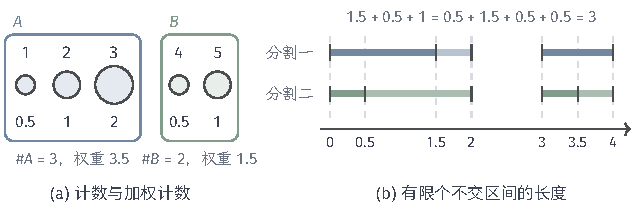
\includegraphics[width=107.6mm]{figures/02-abstract-mathematics/01-metric-and-measure/tikz/c2-count-length/figure.pdf}
  \caption{计数、加权计数与长度遵守同一条不交相加规则。(a)五个点按权重画成大小不同的圆，分成$A=\{1,2,3\}$与$B=\{4,5\}$后，个数$3+2=5$，总权重$3.5+1.5=5$；(b)集合$E=[0,2)\cup[3,4)$的两种不交区间分割，灰色竖线是共同细分的切点，两种分割的长度和都等于$3$。}
  \label{fig:measure-count-length}
\end{figure}

\paragraph{有限的含义}
这里的“有限”限制的是参与分割的区间个数，每个区间中仍有无限多个点。非退化区间不能写成有限个单点的并，因此有限可加性既不会在单点层面产生矛盾，也不提供关于单点分割的任何信息。如果把$[0,1]$看成全部单点$\{x\}$的并，每个单点长度为$0$，而“$0$的不可数和”没有定义，有限可加性根本不适用于这种分割。后面将看到，测度允许的是可数分割：比有限分割多，又比任意不可数分割少，这条界线正是后续理论成立的依据。

\subsection{Jordan测量}
\label{sec:measure-jordan}

有限个不交区间的并只是很少一部分集合。对更一般的有界集合，自然的想法是从里面和外面同时用这类简单集合去逼近。下面把有限个有界区间的并称为\term{初等集合}（elementary set）；它总能改写成有限个不交区间的并，因此上一小节的长度对它有定义。若初等集合$P\subseteq Q$，则$Q\setminus P$仍是初等集合，于是$\ell(P)\le\ell(P)+\ell(Q\setminus P)=\ell(Q)$，长度对包含关系单调；对任意两个初等集合，再由$P\cup Q=P\cup(Q\setminus P)$得$\ell(P\cup Q)\le\ell(P)+\ell(Q)$，并可推广到有限个。

\begin{definition}[Jordan测量]
\label{def:measure-jordan}
设$E\subseteq\mathbb R$有界。称
\[
 \begin{aligned}
  J_*(E)&=\sup\{\ell(P):P\text{为初等集合},\ P\subseteq E\},\\
  J^*(E)&=\inf\{\ell(Q):Q\text{为初等集合},\ E\subseteq Q\}
 \end{aligned}
\]
分别为$E$的\term{Jordan内测量}（Jordan inner content）与\term{Jordan外测量}（Jordan outer content），其中空集作为初等集合长度为$0$。若$J_*(E)=J^*(E)$，称$E$是\term{Jordan可测}（Jordan measurable）的，公共值记为$J(E)$，称为$E$的\term{Jordan测量}（Jordan content）。
\end{definition}

任取内部初等集合$P\subseteq E$与外部初等集合$Q\supseteq E$，有$P\subseteq Q$，由单调性得$\ell(P)\le\ell(Q)$，所以总有$J_*(E)\le J^*(E)$。Jordan可测就是内外两侧可以夹逼到同一个数。这与卷一用有限分割上的上和、下和夹逼定积分是同一种思路（可参考\BookChapterRef{chap:univariate-integration}{卷一“一元积分”章}）：那里固定区间、逼近函数下方的面积，这里固定长度规则、逼近集合本身。

\paragraph{Jordan可测集的例子}
区间$[a,b]$本身是初等集合，内外测量都等于$b-a$。有限个区间的并同理。边界简单的无限集合也可以Jordan可测：取$E=\{1/n:n\ge1\}$，它不含非退化区间，内测量为$0$；对任意$N$与$\varepsilon>0$，用$[0,1/N]$盖住$n\ge N$的全部点，再用长度各为$\varepsilon/N$的小区间盖住$1,1/2,\dots,1/(N-1)$，外部初等集合的长度不超过$1/N+\varepsilon$，令$N\to\infty$、$\varepsilon\to0$得$J^*(E)=0$。可见有限个区间可以覆盖无限多个点，前提是这些点聚集在少数位置附近。

\paragraph{有理点集的反例}
取$E=\mathbb Q\cap[0,1]$。任何非退化区间都含无理数，所以包含在$E$中的初等集合只能由单点组成，长度为$0$，$J_*(E)=0$。另一方面，设初等集合$Q\supseteq E$，把它写成不交区间$I_1,\dots,I_m$的并。把每个$I_k$换成它的闭包$\overline{I_k}$，长度不变，而$\bigcup_k\overline{I_k}$是闭集并包含$E$；$E$在$[0,1]$中稠密，所以这个闭集包含$E$的全部极限点，即包含$[0,1]$。由有限次可加与单调性，$\ell(Q)=\sum_k\ell(\overline{I_k})\ge\ell(\bigcup_k\overline{I_k})\ge\ell([0,1])=1$；而$[0,1]$本身是外部初等集合，故$J^*(E)=1$。内外测量分别为$0$和$1$，$E$不是Jordan可测的。问题出在有限覆盖：有理点到处都是，有限个区间要盖住它们，就不得不连同中间的全部无理数一起盖住。

如果允许可数个区间，情况完全不同。把$E$中的点排成一列$q_1,q_2,\dots$，对给定的$\varepsilon>0$，用长度为$\varepsilon2^{-k}$、以$q_k$为中心的开区间盖住$q_k$。这些区间盖住了$E$，长度总和为$\sum_{k\ge1}\varepsilon2^{-k}=\varepsilon$。图~\ref{fig:measure-jordan-rationals}对比了两种覆盖：有限覆盖必须铺满整个$[0,1]$，可数覆盖的区间越来越短，总长可以任意小。可数覆盖于是给出了另一种测量方式，在它之下有理点集的大小应为$0$。

\begin{figure}[!htbp]
  \centering
  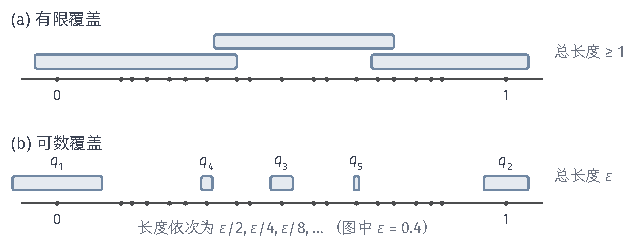
\includegraphics[width=107.8mm]{figures/02-abstract-mathematics/01-metric-and-measure/tikz/c2-jordan-rationals/figure.pdf}
  \caption{用区间覆盖$[0,1]$中的有理点。(a)有限个区间要盖住稠密的有理点，闭包后必须铺满$[0,1]$，总长度不小于$1$；(b)按排列顺序给第$k$个有理点$q_k$分配长度$\varepsilon2^{-k}$的区间，图中只画出前五个，长度依次减半，总长度为$\varepsilon$。}
  \label{fig:measure-jordan-rationals}
\end{figure}

\paragraph{对可数运算的要求}
有理点集还暴露了Jordan测量的另一缺陷。每个单点$\{q_k\}$都Jordan可测且测量为$0$，可是它们的可数并$E$不是Jordan可测的；Jordan可测集合族对可数并不封闭。然而分析中处处需要可数运算：一列集合取并或取交，用逐项逼近得到的集合列求极限，把一个集合分成可数个不交的部分。我们因此提出两项要求。第一，允许测量的集合族应对补集、可数并和可数交封闭；第二，若集合被分成可数个不交的可测部分，整体的大小应等于各部分大小的级数和。这里只提出要求，满足它们的测量规则是否存在、与区间长度是否一致，由第~\ref{sec:measure-construction}节的构造回答。
